\section{Delsystem}

Systemet är indelat i två olika delsystem. Dessa system körs sekvensiellt,
alltså det ena efter det andra. Varje sekund körs de två delsystemen 10 gånger.
Det första systemet kontrollerar själva bilkörningen medan det andra systemet
kontrollerar displayen. Se figur~\ref{fig:system_diagram} för ett processchema.

\begin{figure}
  \centering
  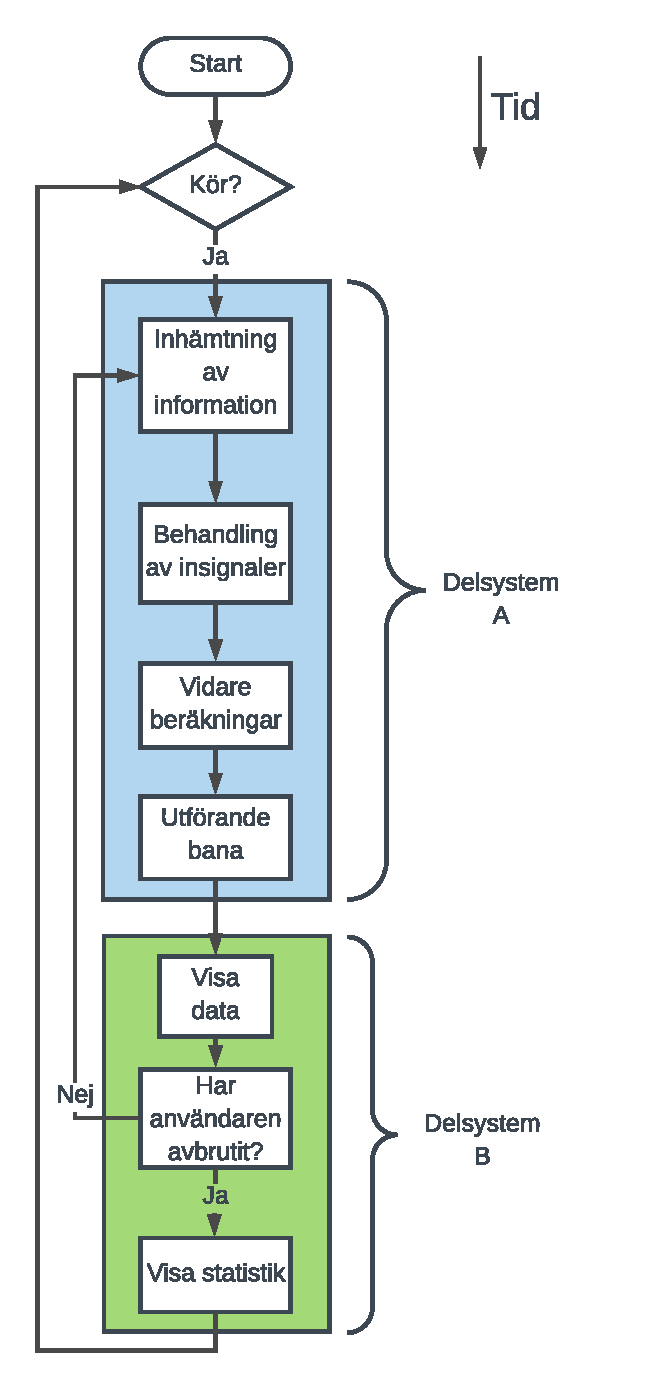
\includegraphics[width=\linewidth,height=0.9\textheight,keepaspectratio]{figures/Processchema.pdf}
  \caption{Processchema över systemets helhet.}%
  \label{fig:system_diagram}
\end{figure}

  \subsection{Delsystem A: Bana}
  
  Delsystem A är indelat i tre övergripande delar. I del A.1 hämtas all
  tillgänglig information in, i del A.2a görs beräkningar utifrån tillgänglig
  data, i del A.2b görs vidare beräkningar (alltså beräkningar som inte baseras
  direkt på den tillgängliga informationen), och i del A.3 utförs de ändringar
  som programmet bedömer är nödvändiga för att klara den valda varvtiden och
  gemensam målgång. 

    \subsubsection{Inhämtning av information}

    Informationen som finns tillgänglig är kraftigt begränsad. I praktiken
    kommer programmet endast fråga om någon av bilarna passerat en givare sedan
    programmet frågade förra gången.

    \subsubsection{Behandling av insignaler}

    De beräkningar som beror direkt på tillgänglig information. Då ny indata
    endast kommer då en bil passerar en givare görs dessa beräkningar inte
    varje cykel.  Ny indata används för att bestämma bilens position och för
    att kalibrera en konstant. Dessa funktioner beskrivs mer ingående i
    \ref{sec:system_a_funcs}.

    \subsubsection{Vidare beräkningar}
    
    Den första beräkningen som görs är bilens nuvarande position. Detta görs
    med hjälp av en intern bild av banan och vetskapen om vilken hastighet och
    position bilen tidigare haft. Sedan beräknas den position som bäst gör att
    bilen klarar den satta varvtiden ut med hjälp av den nuvarande tiden och,
    om gemensam målgång är aktiverat, positionen av den andra bilen.  I början
    av varvet görs inte lika drastiska hastighetsändringar som mot slutet.

    Det sista som händer är att informationen om bilens och banans skick
    används för att räkna ut vilket spänningspådrag som krävs för att få bilen
    att nå den hastighet och position som krävs.

    \subsubsection{Utförande}

    I utförandet skickas det nya spänningspådraget till banorna. 
	
    \subsubsection{Funktioner i delsystem A} \label{sec:system_a_funcs}

    I figur~\ref{fig:flow_diagram} visas flödet av de funktioner som sker i
    delsystem A under en programcykel (alltså 10 gånger per sekund).

    Här listas namn på funktionerna och deras funktion:

    \begin{itemize}
      
      \item old\_v: Bilens hastighet från olika segment, nuvarande varvet och
        tidigare lopp. Från denna databas kan andra funktioner få information
        om hastigheten bilen tidigare haft.
      
      \item old\_position: Bilens tidigare placering. Från denna databas kan
        andra funktioner få information om var bilen var förra cykeln, var
        bilen var för ett varv sedan och så vidare.

      \item indata: Information om huruvida en givare har passerats sedan förra
        cykeln.
      
      \item car\_constant: Påverkar new\_u så att new\_u tillsammans med
        track\_u\_constant motsvarar den hastighet som anges av new\_v.
        car\_constant ändras endast vid ny indata, vilket innebär att den är
        konstant under resterande cykler fram tills nästa givare passeras.
        Genom att jämföra positionen som fås av givarna med indatan kan
        programmet räkna ut felmarginalen som har uppstått och kalibrera
        car\_constant new\_u kan justeras med större precision.
      
      \item position: Var på banan bilen befinner sig. Fås genom att hämta
        senaste positionen (old\_ position) och addera sträckan bilen har
        färdats sedan dess senaste värde. Sträckan som bilen har färdats kan
        räknas ut genom $S = v \cdot \delta t$ där $V = \textrm{old\_v}$ samt
        $\delta t = \textrm{tiden sen senaste cykeln}.$. Om det finns ny indata
        denna cykel är positionen känd och den faktiska positionen används
        istället.
      
      \item clock: Hur länge bilen har varit i det nuvarande segmentet och
        varvet.

      \item car\_position\_diff: Bilarnas position gentemot varandra. Endast
        aktiv om gemensam målgång aktiverad. Funktionen utgår från respektive
        bils placering (old\_position) och hastighet (old\_v) och ger ett värde
        på placeringsskillnaden för en viss hastighet. Detta används för att
        sätta bilarnas nya hastighet. Värdet blir stort om skillnaden i
        placering är stor men justeras också efter hastigeten. Detta betyder
        att om bilarna befinner sig långt ifrån varandra men har en hög
        hastighet blir värdet inte lika stort som om bilarna befinner sig lika
        långt ifrån varandra men har en lägre hastighet. Värdet är positivt om
        bilen på bana 1 ligger före bilen på bana 2 och negativt om bilen på
        bana 2 ligger före bilen på bana 1.  Värdet används sedan för att
        beräkna nästa hastighet (new\_v) som kommer ökas eller minskas för att
        få bilarna att köra ikapp varandra. 

      \item target: Sökt varvtid. Sätts manuellt innan programmet startar.
      
      \item target\_diff: Differensen mellan den önskade tiden och positionen
        relativt till den faktiska tiden och positionen. Fås genom att
        subtrahera de önskade värdena med de faktiska värdena. 
 
      \item agressiveness: Justerar hur stora ändringar som görs på new\_v. Vid
        början av ett varv finns det mycket tid kvar och new\_v kan ändras lite
        i taget istället för att göra stora förändringar direkt. Det är även
        onödigt att göra stora ändringar om bilarna befinner sig ungefär där de
        bör vara. agressiveness räknas ut via clock, hur mycket av varvtiden
        som återstår, target\_diff och hur långt ifrån målet bilen befinner
        sig. Om gemensam målgång är aktiv tas även hänsyn till
        car\_position\_diff.

      \item u\_constant\_map: En kartläggning över banan och de spänningsnivåer
        som behöver sättas så att spänningen blir jämn. Behövs eftersom
        spänningstillförseln beter sig olika vid olika delar av banan.
        Kartläggningen bygger på det register med inlagrad data som tas fram
        genom tester.
    
      \item target\_diff: Bilens position relativt till var den borde befinna
        sig vid den nuvarande tiden.
      
      \item track\_u\_ constant: Det förbestämda spänningsvärdet för ett visst
        subsegment på banan. Tas fram manuellt genom prövning och lagras i
        u\_constant\_map. Från position tar track\_u\_constant fram rätt
        spänningsvärde.
     
      \item speed\_map: En kartläggning över banan och hur över hur fort man
        kan köra i olika delar av banan. Kartläggningen bygger på det register
        med inlagrad data som tas fram genom tester.

      \item speed\_max: Den förbestämda maxhastigheten för nuvarande
        subsegment. Tas fram manuellt genom prövning och lagras i speed\_map.
        Från position tar speed\_constant fram rätt hastighet. 

      \item new\_v: Den hastighet som bilen ska få nästa cykel. Tar förra
        cykelns hastighet (old\_ v) och lägger till eller drar av beroende på
        hur långt ifrån målet bilarna ligger (target\_diff) och, om gemensam
        målgång är aktiverad, hur långt ifrån varandra bilarna är
        (car\_position\_diff). Beror också på agressiveness; högre
        agressiveness ger större skillnad mellan new\_v och old\_v medan ett
        lågt värde gör att new\_v inte ändras särskilt mycket.  new\_v används
        sedan för att sätta new\_u. Högre new\_v ger högre new\_u och lägre
        new\_v ger lägre\_u. 
	
      \item new\_u: Den spänning som ska appliceras beroende på vilken
        hastighet new\_v anger. Ett högre new\_v innebär ett högre new\_u. De
        andra parametrarna som påverkar new\_u är car\_constant och
        track\_u\_constant, desto högre dessa värden dessa antar desto högre
        värde antar också new\_u.  new\_u är programmets sista output, dess
        värde 0 till 127 är det gaspådrag som appliceras på bilen.
    
    \end{itemize}

    \begin{figure}
      \centering
      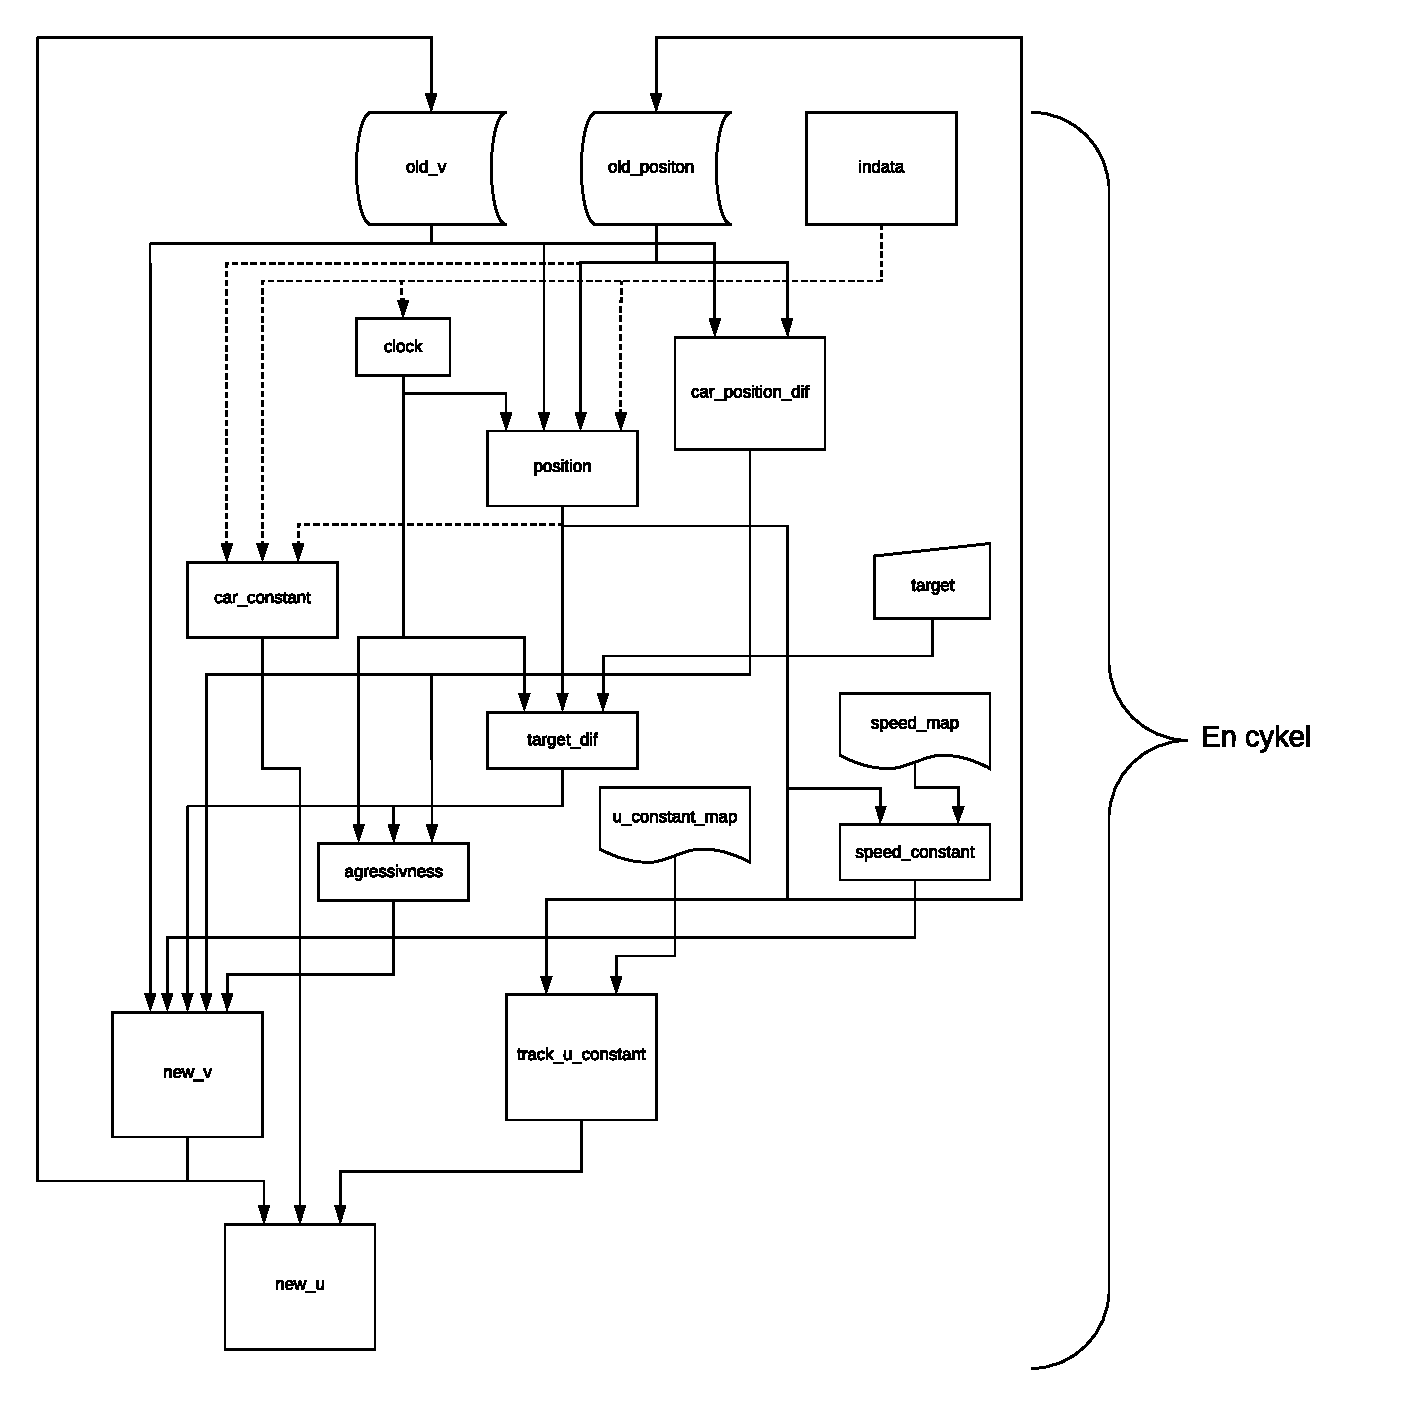
\includegraphics[width=\linewidth]{figures/flow.pdf}
      \caption{Funktionsflödet i delsystem A.}%
      \label{fig:flow_diagram}
    \end{figure}

    \subsection{Delsystem B: Display}

    Displayen ter sig enklare än delsystem A. Under körning ska, om ett nytt varv
    påbörjats, den senaste varvtiden och varvnumret skickas till displayen. Om
    stopp-knappen har tryckts ned ska systemet hoppa till resultat-skärmen och om
    inte så ska det fortsätta.

